\section{Walks}

\frame{
{Part 2: Walks in Graphs}

\tableofcontents[currentsection,hideallsubsections, firstsection=1, sections={1-3}]
}

\subsection{Walks, Paths and Relations}

\begin{frame}[t]{A solution to a problem can be a set of edges and vertices}

{\bf Question:} Is it possible to graduate in the curriculum below?
\begin{tabular}{p{.1\textwidth}|p{.45\textwidth}||p{.3\textwidth}}
  \hline
  Code & Lecture & Prerequisites \\
  \hline
  0000 & {\small Social Questions} & \emph{none} \\
  0001 & {\small Intro to Programming} & \emph{none} \\
  0002 & {\small Calculus I} & \emph{none} \\
  0003 & {\small Programming Theory} & \emph{0001} \\
  0004 & {\small Linear Algebra} & \emph{0000, 0002} \\
  0005 & {\small Programming Challenges} & \emph{0000, 0001, 0003} \\
  0006 & {\small Computer Graphics} & \emph{0003, 0004} \\
  \hline
\end{tabular}\bigskip 

{\bf Answer:} Create the \emph{curriculum's graph} and find a way to go to all vertices from the starting ones.


\end{frame}


\begin{frame}[t]{Walks and Paths}

  The solution of many graph problems is represented as a sequence of vertices and edges.\bigskip 

  A sequence of vertices in a graph is a \structure{Walk} or a \structure{Path}.\bigskip

  \begin{itemize}
    \item {\bf Walk:} Any sequence of successive edges. 

    \item {\bf Path:} A walk that never visits the same vertex more than once.
  \end{itemize}
\end{frame}

\begin{frame}{Walk example}

  \begin{center}
    \begin{tikzpicture}[scale=1.2,auto,swap]
      \tikzset{edge/.style = {->,>=latex'}}
      \node[vertex] (a) at (0,1) {a};
      \node[vertex] (b) at (0,0) {b};
      \node[vertex] (c) at (0,-1) {c};
      \node[vertex] (d) at (2,0) {d};
      \node[vertex] (e) at (3,1) {e};
      \node[vertex] (f) at (3,-1) {f};
      \draw[edge] (a) to (b);
      \draw[edge] (c) to (b);
      \draw[edge] (b) to (d);
      \draw[edge] (d) to (a);
      \draw[edge] (c) to (d);
      \draw[edge] (d) to (e);
      \draw[edge] (e) to (f);
      \draw[edge] (f) to (d);
  \end{tikzpicture}
  \end{center}

  \bigskip

  \begin{block}{Walk: any sequence of successive edges}

    \begin{tikzpicture}[scale=1,auto,swap]
      \tikzset{edge/.style = {->,>=latex'}}
      \node[vertex] (a) at (0,0) {b};
      \node[vertex] (b) at (1,0) {d};
      \node[vertex] (c) at (2,0) {e};
      \node[vertex] (d) at (3,0) {f};
      \node[vertex] (e) at (4,0) {d};
      \node[vertex] (f) at (5,0) {e};
      \draw[edge] (a) to (b);
      \draw[edge] (b) to (c);
      \draw[edge] (c) to (d);
      \draw[edge] (d) to (e);
      \draw[edge] (e) to (f);
    \end{tikzpicture}

    \begin{itemize}
    \item {\bf Walk lengh:} 5 edges (The length of a walk is the EDGES, not the VERTICES)
    \item {\bf Representing as a compound relation:} $E(E(E(E(E(a)))))$
    \item NOTE: a walk can repeat edges and vertices! 
    \end{itemize}
  \end{block}

\end{frame}

\begin{frame}
  \frametitle{Path example}

  \begin{center}
    \begin{tikzpicture}[scale=1.2,auto,swap]
      \tikzset{edge/.style = {->,>=latex'}}
      \node[vertex] (a) at (0,1) {a};
      \node[vertex] (b) at (0,0) {b};
      \node[vertex] (c) at (0,-1) {c};
      \node[vertex] (d) at (2,0) {d};
      \node[vertex] (e) at (3,1) {e};
      \node[vertex] (f) at (3,-1) {f};
      \draw[edge] (a) to (b);
      \draw[edge] (c) to (b);
      \draw[edge] (b) to (d);
      \draw[edge] (d) to (a);
      \draw[edge] (c) to (d);
      \draw[edge] (d) to (e);
      \draw[edge] (e) to (f);
      \draw[edge] (f) to (d);
  \end{tikzpicture}
  \end{center}

  \begin{block}{Path: A walk without repeated vertices}

    \begin{tikzpicture}[scale=1,auto,swap]
      \tikzset{edge/.style = {->,>=latex'}}
      \node[vertex] (a) at (0,0) {e};
      \node[vertex] (b) at (1,0) {f};
      \node[vertex] (c) at (2,0) {d};
      \node[vertex] (d) at (3,0) {a};
      \node[vertex] (e) at (4,0) {b};
      \draw[edge] (a) to (b);
      \draw[edge] (b) to (c);
      \draw[edge] (c) to (d);
      \draw[edge] (d) to (e);
    \end{tikzpicture}\hspace{1cm} {\bf Stuck!}

    \begin{itemize}
    \item {\bf Path lengh:} 4 edges (The length is counted in EDGES, not vertices)
    \item {\bf \structure{Eulerian Walk:}} Every \structure{edge} is visited once ({\bf E}ulerian).
    \item {\bf \alert{Hamiltonian Path:}} Every \alert{vertex} is visited once.
    \item {\bf Eulerian / Hamiltonian Circuit}: You go back to the initial vertex
    \end{itemize}
  \end{block}
\end{frame}

\begin{frame}{Proofs with Walks and Paths}
  \begin{proof}[Proof: The shortest Walk between two vertices is a Path]
    {\bf Proof by contradiction:} Assume a shortest walk that is not a path.

    \begin{enumerate}
    \item The shortest walk between $v_0$ and $v_n$ is not a path. So it has a repeated vertice $v_k$:
    \begin{equation*}
      w_{0,n} = v_0 \to v_1 \to \ldots \to v_k \to \ldots \to v_k \to \ldots \to v_{n-1} \to v_n
    \end{equation*}

    \item $w_{0,n}$  contains a smaller walk $w_{k,k}$ from $v_k$ to $v_k$ of size $|w_{k,k}| \geq 1$.
    \item We can remove $w_{k,k}$ from $w_{o,n}$, resulting in a smaller walk $w_{0,2}'$ with size $|w_{0,n}| - |w_{k,k}|$
    \item $w_{0,n}'$ is a walk from $v_0$ to $v_n$ that is shorter than $w_{0,n}$, which is a contradiction.
    \end{enumerate}
  \end{proof}

  This can be used to prove the \structure{Triangle Inequality} in walks (the distance of $i,j$ is equal or smaller than the distance from $i,k$ + $k,j$)

\end{frame}

\begin{frame}[t]{The Walk Relation}

  Let's describe a binary relation between vertices $v_i$ and $v_j$ in graph $G$,\\ and call it the \structure{Walk Relation}: 
  \begin{equation*}
    v_i G^n v_j.
  \end{equation*}

  The relation $G^n$ means: "There is a walk from $v_i$ to $v_j$ with length exactly $n$."\bigskip

  Let's think about $G^n$:
  \begin{itemize}
    \item $G^0$ is the set of all vertices (walk of size 0 goes nowhere)
    \item $G^1$ is the set of all pairs of vertices connected by 1 edge    
    \item {\bf composition and addition:} $G^n \circ G^m = G^{n+m}$ \hspace{.5cm}\\
    (For example, $G^2 + G^3 = G^5$)
    \item {\bf common vertex:} If there is a composite relation between $v_x$ and $v_y$ ($v_x~G^m \circ G^n~v_y$), this implies that there is a common vertex connecting them:\\
    $v_x~G^m \circ G^n~v_y\rightarrow \exists z, v_x~G^m~v_k, v_k~G^n~v_y$

  \end{itemize}
\end{frame}

\begin{frame}[t]{The Walk Relation and the Adjacency Matrix}

  Before, we described the Adjacency Matrix $A$, where $A_{i,j}=1$ if $E(v_i$,$v_j)$.
  \bigskip
  
  If we rename $A$ to $A_{G^1}$, we can generalize this concept to the \structure{Walk Matrix $A_{G^n}$}, which is the adjacency matrix representing $G^n$: $A_{G^n,i,j}=1$ if $v_i~G^n~v_j$. ($\exists$ walk of size $n$ from $v_i$ to $v_j$)
  \bigskip

  It is possible to calculate $A_{G^n}$ using \emph{boolean matrix multiplication}: $A_{G^n\circ G^m} = A'_{G^n} \odot A''_{G_m}$:

  \begin{equation*}
    a_{ij} = A'_{i*} \odot A''_{*j} = (a'_{i0} \land a''_{0j}) \lor (a'_{i1} \land a''_{1j}) \lor (a'_{i2} \land a''_{2j}) \lor \ldots \lor (a'_{in} \land a''_{nj})
  \end{equation*}\medskip

  This means that we can calculate $A_{G^n}$ quickly using the \structure{Fast Matrix Exponentiation}:

  \begin{itemize}
    \item $A_{G^n} = A_{G^{n/2}} \odot A_{G^{n/2}} = (A_{G^{n/4}} \odot A_{G^{n/4}}) \odot (A_{G^{n/4}} \odot A_{G^{n/4}}) = \ldots$
  \end{itemize}

\end{frame}

\begin{frame}[t]{Walk Relation $G^*$ of a Digraph}

  \begin{itemize}
  \item $G^n$ is the \structure{length $n$ walk relation}: It representes \structure{all walks of size exaclty $n$}
  \item $G^*$ is the \alert{walk relation of $G$}: It representes \alert{all walks in $G$}.
  \item $u G^* v$ means that \alert{there is a walk of {\bf some} length from $u$ to $v$}\\
  \end{itemize}\bigskip

  \structure{QUIZ:} How do we calculate $A_{G^*}$ for a graph, given adjacency matrix $A_{G^1}$?\bigskip

  \alert{HINT:} Remember that a walk can be infinite. But we need to solve this problem with a {\bf finite} algorithm! When does the algorithm stop?
\end{frame}

\begin{frame}[t]{Walk Relation of a DiGraph}{How to calculate $G^*$}

  \begin{enumerate}
  \item Let $G^1$ be the relation defined by the original graph (or its adjacency matrix).\medskip

  \item Let $G^0$ be the relation defined by the set $V$ with self:
    \begin{tikzpicture}[scale=1.5,auto,swap]
      \tikzset{edge/.style = {->,>=latex'}}
      \node[vertex] (a) at (0,0) {};
      \draw[edge] (a) to[loop left] (a);
    \end{tikzpicture}\\
    ($A_{G^0}$: the identity matrix).\medskip

  \item The relation $G^{\leq 1} = G^0 \cup G^1$ is the relation for walks of \emph{length 1 or less};\\
  ($A_{G^\leq 1} = A_{G^0} \times A_{G^1}$)\medskip

  \item $G^* = (G^{\leq})^{n-1}$: All walks of size $n-1$ or less.\hfill ({\bf Q: Why not n?})\medskip 
  
  \item Using fast exponentiation, you can calculate $G^*$ in $\log n$ matrix boolean multiplications
  \end{enumerate}
\end{frame}

\begin{frame}[t]{Adjacency Matrices and Neural Networks}{Why did we just study this?}
  We just studied an algorithm that can quickly calculate all the walks in a directed graph.\bigskip 

  If the graph is also {\bf acyclic}, and the edges have {\bf weights} in them, this algorithm can be easily generalized to \structure{calculate the total weight between any two vertices}.\bigskip 

  This can be used to quickly calculate the weight between the input neuron and the output neuron of a very large network!\bigskip

  \structure{This is one reason why Matrix Multiplications are important for Machine Learning.}

  \vfill 
  (caveat emptor: it gets more complicated with loops, non-linear activation functions, etc)
\end{frame}

\subsection{Prerequisite Course Graphs}

\begin{frame}{Walks and Prerequisite Course Graphs}
  \begin{columns}
    \column{0.4\textwidth}
      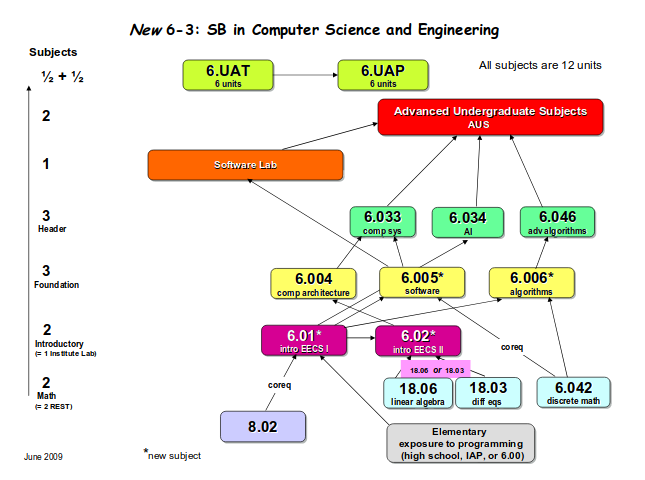
\includegraphics[width=1\textwidth]{../img/MIT_prereq}
      \pagenote{Course Pre-requisite image from "Math for CS" MIT OCW}
    \column{0.6\textwidth}
      The \emph{walk relation} of the pre-requisite graph $R$ defines how the courses relate to each other.
      \begin{itemize}
      \item \structure{Direct Prerequisite}: Req(6.046) = 6.006
      \item \structure{Indirect Prerequisite}: Req(6.046) = $\{6.006, 6.042, 6.01, 6.00, 8.02\}$
      \end{itemize}\medskip
  \end{columns}\bigskip

  Course $u$ is an indirect prerequisite of $v$ if there is a positive length walk from $u$ to $v$ in $R$:\medskip

  \begin{equation*}
    u D^+ v
  \end{equation*}
\end{frame}

\begin{frame}
  \frametitle{Requisites, Cycles and DAGs}

  In the beginning of the lecture, we talked about a prerequisite graph where it was not possible to graduate. Why? Because it had {\bf cycles}.\medskip

    \begin{itemize}
    \item A \structure{closed walk} is a walk that starts and ends at the same vertex.\medskip

    \item A \structure{cycle} is a closed walk where the only repeat
      vertex is at the beginning and end.
      \begin{itemize}
        \item $v_0 \to v_1 \to \ldots \to v_n \to v_0 | i > 0, j > 0, v_i \neq v_j$
        \item A cycle is the path $v \to w + (w,v)$
      \end{itemize}\medskip

    \item A \alert{Directed Acyclic Graph (DAG)} is a digraph that has
      \structure{no positive length cycles}.
    \end{itemize}
\end{frame}

\begin{frame}{Directed Acyclic Graphs Examples}

  Directed Acyclic Graphs (DAGs), can be used to represent several ordered structures:

    \begin{itemize}
      \item Course Prerequisite Graphs;
      \item Ordered Task List:
      \begin{itemize}
        \item "first add rice, then add water, then press cook button"
        \item "Let x be 5, let y be 2, while y $>$ 0, multiply x by x and subtract 1 from y."
      \end{itemize}
    \end{itemize}
    \bigskip

  Computational structures can also be described using DAGs:\medskip

    \begin{itemize}
      \item Relations, for example:
      \begin{itemize}
        \item \structure{Successor Relation}: $n \to n+1$
        \item \structure{Subset Relation}: $\{1,2\} \subset \{1,2,3\}$
      \end{itemize}
      \item Induction Proofs: ($P(n) \implies P(n+1) \implies P(n+2) \ldots$);
      \item Dynamic Programming: (base cases and transitions on the DP table);
    \end{itemize}
\end{frame}

\begin{frame}
  \frametitle{Directed Acyclic Graphs (DAG) and covering edges}

  \begin{columns}
    \column{0.3\textwidth}
    \begin{tikzpicture}[scale=.5,auto,swap]
      \tikzset{edge/.style = {->,>=latex'}}
      \node[vertex] (a) at (2,5) {a};
      \node[vertex] (b) at (1,3) {b};
      \node[vertex] (c) at (3,3) {c};
      \node[vertex] (d) at (2,2) {d};
      \node[vertex] (e) at (0,0) {e};
      \node[vertex] (f) at (4,0) {f};
      \draw[edge] (a) to (b);
      \draw[edge] (a) to (c);
      \draw[edge] (a) to (d);
      \draw[edge] (c) to (f);
      \draw[edge] (d) to (f);
      \draw[edge] (c) to (d);
      \draw[edge] (b) to (d);
      \draw[edge] (a) to[bend right] (e);
      \draw[edge] (a) to[bend left] (f);
      \draw[edge] (b) to[bend right] (f);
    \end{tikzpicture}

    \begin{tikzpicture}[scale=.5,auto,swap]
      \tikzset{edge/.style = {->,>=latex'}}
      \node[vertex] (a) at (2,5) {a};
      \node[vertex] (b) at (1,3) {b};
      \node[vertex] (c) at (3,3) {c};
      \node[vertex] (d) at (2,2) {d};
      \node[vertex] (e) at (0,0) {e};
      \node[vertex] (f) at (4,0) {f};
      \draw[edge] (a) to (b);
      \draw[edge] (a) to (c);
      \draw[edge] (d) to (f);
      \draw[edge] (c) to (d);
      \draw[edge] (b) to (d);
      \draw[edge] (a) to[bend right] (e);
    \end{tikzpicture}

    \column{0.7\textwidth}

      Given a DAG $A$, its \structure{covering edges} is the {\bf smallest} DAG $B$ that has the same \structure{Walk Relation} as $A$\bigskip

      Walk relation of $A$ and $B$:
      \begin{itemize}
      \item $a\to \{b,c,d,e,f\}$
      \item $\{b,c\}\to \{d,f\}$
      \item $d\to f$
      \item $\{e,f\} \to \emptyset$
      \end{itemize}
  \end{columns}
\end{frame}
